\section{Performance and scaling}
\label{sec:scaling}

All compute timings are on one host, \texttt{rosi\_v100} (node
\texttt{gv002}), exclusive Slurm allocation, pinned to GPU 0. Build: CUDA
12.6, \texttt{PICBUNCH\_ARCH=70}, Release, padding 2, double. Each
configuration ran three timed repeats after one untimed warm-up plus one
device-level warm-up; stage values are medians, the total is
min/median/max. The four $\gamma=10$, $N=2\times10^6$ repeats give total
medians $60.35$ to $64.76$ ms, about $7\%$ scatter; the $64.81$ ms row is
the $\gamma=100$ run. These compute-only totals exclude the checkpoint
writer; the end-to-end totals with the writer are in Table~\ref{tab:e2e},
a different measurement path.

\paragraph{Reproducibility.}
The matrix of Table~\ref{tab:matrix} is the \texttt{picBunchBench} sweep,
run with
\seqsplit{picBunchBench --sweep --repeat 3 --csv matrix.csv}. The input
bunches are not checked into the repository; the sweep configuration is the
generator. The fast GPU kernel
\seqsplit{tools/closed-form/gpu\_extract.cu} is part of the source.
The H100 runs used CUDA $13.4$.

\paragraph{Correctness anchor.}
Every timing run is anchored by the Coulomb limit ($\mathbf{u}=0$): one
particle at a node, far nodes at $d=8,16,24,32$ along all six axis
directions. The mesh field against the direct TSC stencil sum of the
analytic Coulomb kernel has worst relative error $4.88\times10^{-14}$ (max
absolute $2.28\times10^{-25}$), passing the $10^{-12}$ threshold. This
confirms that the zero-padded FFT convolution reproduces the TSC-convolved
Coulomb field to roundoff (Section~\ref{sec:consistency}).

\begin{figure}[t]
\centering
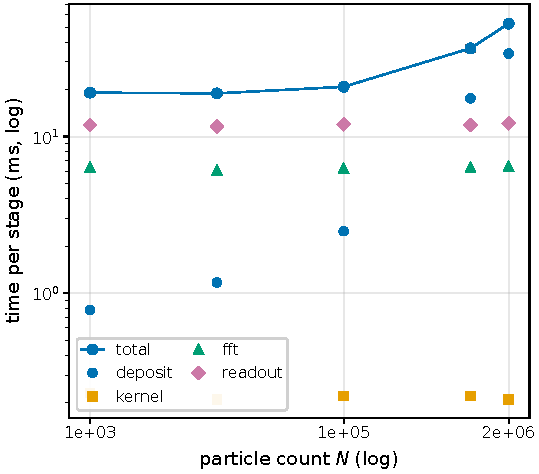
\includegraphics[width=0.62\linewidth]{figs/F_a_scaling_vs_N.pdf}\\[2pt]
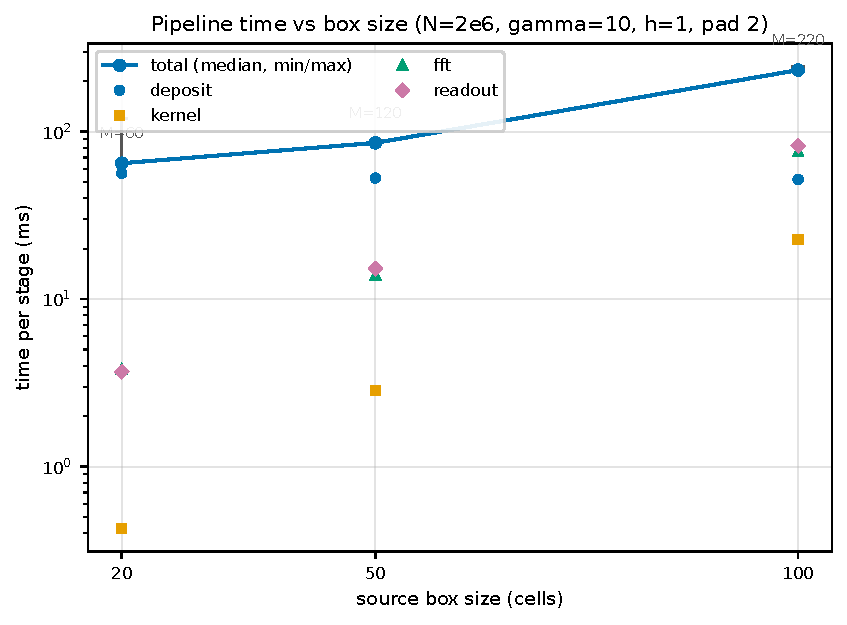
\includegraphics[width=0.62\linewidth]{figs/F_b_scaling_vs_box.pdf}
\caption{Pipeline time versus particle count (top, log-log) and source-box
size (bottom, semi-log), padded array $M=60/120/220$ cells, $\gamma=10$,
$h=1$, double precision, \texttt{rosi\_v100}/CUDA 12.6. Blue is the total
and markers the per-stage medians; the deposit dominates at
$N=2\times10^6$ ($57$ of $64.8$\,ms), and the total rises from $64.8$ to
$233$\,ms as $M$ grows from $60$ to $220$.}
\label{fig:Fa}
\end{figure}

Figure~\ref{fig:Fa} sweeps one axis at a time: the top panel fixes the
20-cell box and varies $N$, the bottom panel fixes $N=2\!\cdot\!10^6$ and
varies the box. The scaling is in two regimes, with the crossover set by
the box, not the particle count. At large $N$ the deposit dominates, linear
in $N$, $52$--$57$ ms on the $2\times10^6$ rows while the FFT, kernel, and
read-out stay under $10$ ms at the $20$-cell box; the total is flat across
$\gamma=1,10,100$ ($64.9/64.4/64.8$ ms). At large boxes the kernel and FFT
scale with $M^3$: from $M=60$ to $M=220$ the total goes from $64.8$ ms to
$233$ ms, and halving $h$ costs $1.07\times$ and $2.35\times$ because the
deposit stays constant. The per-$h$ totals are $64.76$, $69.27$, and
$151.51$ ms for $h=1$, $1/2$, $1/4$ (padded array $M=60/100/180$,
$2\times10^6$ particles, 20-cell box). On the H100 (\texttt{jrc0880},
\texttt{sm\_90}), the same $2\times10^{6}$, $20$-cell, $h=1$ mesh is
$0.052$\,s compute (deposit $34.4$\,ms, kernel $1.08$\,ms, FFT $7.44$\,ms,
read-out $9.02$\,ms; medians of three), and $0.755$\,s CLI wall including
the particle read and the HDF5 write.

\begin{table}[t]
\centering
\small
\caption{Per-stage medians (ms) and device allocation (MiB), padding 2,
double, \texttt{rosi\_v100} GPU 0. ``box'' is the source-box size in cells;
$M$ is the padded FFT array per axis. Stage columns are medians over the
three timed repeats.}
\label{tab:matrix}
\begin{tabular}{lrrrrrrrrrrr}
\toprule
$N$ & box & $\gamma$ & $h$ & $n$ & $M$ & total & deposit & kernel & FFT & read-out & dev \\
\midrule
$10^3$   & 20  & 10  & 1   & 30  & 60  & 10.17  & 1.13  & 0.48 & 4.36  & 4.08  & 8.4  \\
$10^4$   & 20  & 10  & 1   & 30  & 60  & 10.69  & 2.42  & 0.53 & 4.37  & 3.35  & 8.7  \\
$10^5$   & 20  & 10  & 1   & 30  & 60  & 12.90  & 4.59  & 0.48 & 4.07  & 3.28  & 11.4 \\
$10^6$   & 20  & 10  & 1   & 30  & 60  & 61.92  & 53.61 & 0.53 & 4.31  & 3.45  & 38.9 \\
$2\!\cdot\!10^6$ & 20  & 10  & 1   & 30  & 60  & 64.76  & 56.51 & 0.43 & 3.80  & 3.69  & 69.4 \\
$2\!\cdot\!10^6$ & 50  & 10  & 1   & 60  & 120 & 85.67  & 52.82 & 2.85 & 13.89 & 15.20 & 127.4 \\
$2\!\cdot\!10^6$ & 100 & 10  & 1   & 110 & 220 & 232.97 & 51.89 & 22.66 & 75.97 & 82.40 & 468.7 \\
$2\!\cdot\!10^6$ & 20  & 10  & 1/2 & 50  & 100 & 69.27  & 52.38 & 1.29 & 7.43  & 8.16  & 99.5  \\
$2\!\cdot\!10^6$ & 20  & 10  & 1/4 & 90  & 180 & 151.51 & 50.94 & 11.76 & 43.38 & 44.58 & 284.5 \\
\bottomrule
\end{tabular}
\end{table}

No configuration came near the $32$ GB device limit; the largest exact
device allocation was $468.7$ MiB. Memory scales with the padded bunch box,
not the global field.

\begin{table}[t]
\centering
\small
\caption{End-to-end pipeline time including the checkpoint writer and the
openPMD reader, medians over 3 repeats, \texttt{rosi\_v100} GPU 0, 20-cell
box, $\gamma=10$, CLI \texttt{--tolerance} $10^{-3}$. A different
measurement path from the compute-only Table~\ref{tab:matrix}: the totals
include the writer (the dominant added term); the per-stage split is
deposit/kernel/FFT/readout/writer.}
\label{tab:e2e}
\begin{tabular}{lrrrrrr}
\toprule
$N$ & total & deposit & kernel & FFT & readout & write \\
\midrule
$10^{4}$  & 22.00 & 2.70  & 0.53 & 4.53 & 3.06 & 11.29 \\
$10^{5}$  & 24.87 & 5.82  & 0.56 & 4.31 & 3.80 & 10.65 \\
$10^{6}$  & 47.15 & 31.56 & 0.46 & 4.20 & 3.95 & 7.54  \\
\bottomrule
\end{tabular}
\end{table}

Table~\ref{tab:e2e} is the same pipeline with the writer in the loop. The
deposit is still linear in $N$ ($2.70\to31.56$ ms from $10^4$ to $10^6$),
and the FFT is still box-bound and flat. The writer is the dominant added
term: $11.29$ ms at $10^4$ and $7.54$ ms at $10^6$. The $N=10^6$ total is
$47.15$ ms with the writer, versus $61.92$ ms in the compute-only
Table~\ref{tab:matrix}; the two campaigns differ in measurement path and
timing boundary, so neither is the other's total plus the writer.

\subsection{MPI rank scaling}
\label{sec:mpi-scale}

The rank-parallel compute and the collective writer were remeasured on
\texttt{jureca-h100} (four H100 PCIe 80\,GB, sm\_90, CUDA 13.4,
medians of three serialized runs).  The mesh stage
(deposit + kernel + FFT + read-out) at $N=2\times10^{6}$, $256^3$ takes
$581$, $411$ and $325$\,ms at $1$, $2$ and $4$ ranks ($1.41\times$ and
$1.79\times$); the replicated deposit and source spectrum cap the speedup.
The fast-GPU near shell at $32^3$, $R=1.5$, tile 8 takes $519$, $653$ and
$1112$\,ms: at this small size the tile split and the correction all-reduce
dominate, so more ranks do not help.  The collective HDF5 writer at
$256^3$ takes $3319$, $3327$ and $3323$\,ms at $1$, $2$ and $4$ ranks
($1.00\times$), essentially flat and the dominant part of the total.

\begin{table}[t]
\centering
\small
\caption{Rank scaling on \texttt{jureca-h100}, medians of three serialized
runs.  Mesh: $N=2\times10^{6}$, $256^3$, component-parallel (replicated
deposit and source FFT).  Near shell: $N=200$, $32^3$, $R=1.5$, tile 8,
tile-parallel, fast-GPU.  Write: $256^3$, collective HDF5.  The near-shell
column is a small-size case where the all-reduce dominates; the mesh and
writer are the production-relevant columns.}
\label{tab:mpi}
\begin{tabular}{lccc|cc|cc}
\toprule
 & \multicolumn{3}{c}{near shell} & \multicolumn{2}{c}{mesh} & \multicolumn{2}{c}{write} \\
\cmidrule(lr){2-4}\cmidrule(lr){5-6}\cmidrule(lr){7-8}
ranks & wall (ms) & speedup & eff.\ & wall (ms) & speedup & wall (ms) & speedup \\
\midrule
1 & $519.4$ & $1.00$ & $100\%$ & $581$ & $1.00$ & $3319$ & $1.00$ \\
2 & $652.9$ & $0.80$ & $40\%$  & $411$ & $1.41$ & $3327$ & $1.00$ \\
4 & $1112.2$ & $0.47$ & $12\%$ & $325$ & $1.79$ & $3323$ & $1.00$ \\
\bottomrule
\end{tabular}
\end{table}

\begin{figure}[H]
\centering
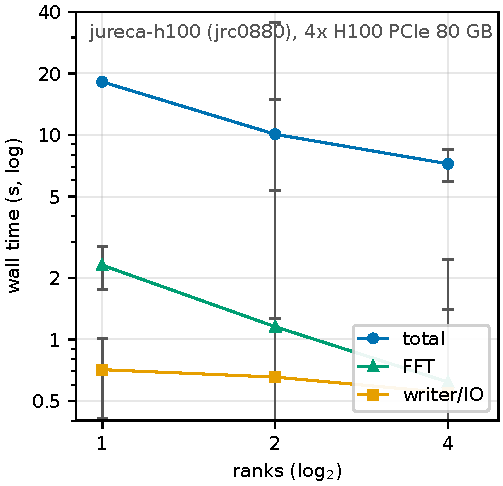
\includegraphics[width=0.58\linewidth]{figs/F_mpi_rank_scaling_h100.pdf}
\caption{Strong scaling of the three rank-parallel pieces on
\texttt{jureca-h100} for $1$--$4$ ranks, medians of three serialized runs:
near shell ($32^3$, $R=1.5$, tile 8), mesh ($2\times10^{6}$ particles,
$256^3$), and the collective writer ($256^3$).  The writer is flat; the
mesh reaches $1.79\times$; the small near-shell case has all-reduce
overhead and does not scale.}
\label{fig:h100mpiscaling}
\end{figure}

\paragraph{Distributed-mode scaling and its limits.}
The writer column above is the replicated path: only rank 0 writes the full
field, so it cannot scale by construction.  Forcing the slab-local production
mode (\texttt{--fft-mode distributed}) at $256^3$, $N=2\times10^{6}$, gives a
total of $21.6$, $12.3$ and $13.0$\,s and a writer of $4.19$, $2.88$ and
$6.46$\,s at $1$, $2$ and $4$ ranks; the FFT is $2.30$, $1.16$ and
$0.63$\,s.  The writer scales to two ranks ($1.45\times$) and regresses at
four ($0.65\times$), a collective-HDF5 contention on the shared series, not a
serialisation in picBunch.  The near shell partitions tiles but still
all-reduces the full correction array; at $32^3$ that communication and the
tile imbalance dominate, which is why the near-shell column reverses.  A
local-slab reduction and a writer with per-rank contiguous slabs are the
required fixes for many-rank runs.

\begin{table}[t]
\centering
\small
\caption{Distributed-mode strong scaling, $256^3$, $N=2\times10^{6}$,
medians of three serialized runs.  The writer is the collective HDF5 series;
the replicated writer (only rank 0 writes) is flat by construction and is not
shown here.}
\label{tab:h100dist}
\begin{tabular}{lrrr}
\toprule
 & 1 rank & 2 ranks & 4 ranks \\
\midrule
total (s)   & $21.6$ & $12.3$ & $13.0$ \\
FFT (s)     & $2.30$ & $1.16$ & $0.63$ \\
writer (s)  & $4.19$ & $2.88$ & $6.46$ \\
\bottomrule
\end{tabular}
\end{table}

\subsection{H100 remeasurement}
\label{sec:h100}

A fresh campaign on \texttt{jureca-h100} (four H100 PCIe 80\,GB, sm\_90,
CUDA 13.4, serialized on one GPU, medians of three runs) reproduces the
scaling picture with current hardware.  At $N=2\times10^{6}$, a 20-cell box
takes $60.5$\,ms end to end (deposit $36.1$, FFT $1.53$, read-out $17.5$,
writer $5.1$\,ms); a 100-cell box takes $147.9$\,ms (deposit $38.9$, FFT
$31.3$, read-out $21.4$, writer $53.8$\,ms).  The deposit remains linear in
$N$; the 100-cell case is FFT- and writer-bound.  For $N=200$ particles the
16- and 64-bin multi-velocity runs take $92.2$ and $100.6$\,ms; the $B_z$
peak differs by $4.6\%$, within the shot noise of 200 particles.

Rank scaling at $N=2\times10^{6}$ and the near-shell case are in
Section~\ref{sec:mpi-scale}: the shared HDF5 writer dominates the total and
is flat across ranks, while the mesh stage reaches $1.79\times$ at four
ranks.

\begin{table}[t]
\centering
\small
\caption{H100 remeasurement, medians of three serialized runs.  Top:
$N=2\times10^{6}$, one bin, one rank, stage times in ms.}
\label{tab:h100}
\begin{tabular}{lrrrrr}
\toprule
box & deposit & FFT & read-out & writer & total \\
\midrule
20 cells  & $36.1$ & $1.53$ & $17.5$ & $5.1$  & $60.5$ \\
100 cells & $38.9$ & $31.3$ & $21.4$ & $53.8$ & $147.9$ \\
\bottomrule
\end{tabular}

\end{table}
